\subsection{Deduplication ratio}
\label{sec:dedup_ratio}

%\subsection{Overview of file duplicates}
%\paragraph{File repeat count}
\paragraph{Full file duplicates}
As discussed in compression ratio analysis, we see that there is redundant data in both layers and images.
A simple duplication is to replicate full content of a file. To find out if how many full file duplicates in the dataset, we calculated a digest of the complete file. 
%We conducted simple form of deduplication to  
Interestingly,

\begin{figure}
	\centering
	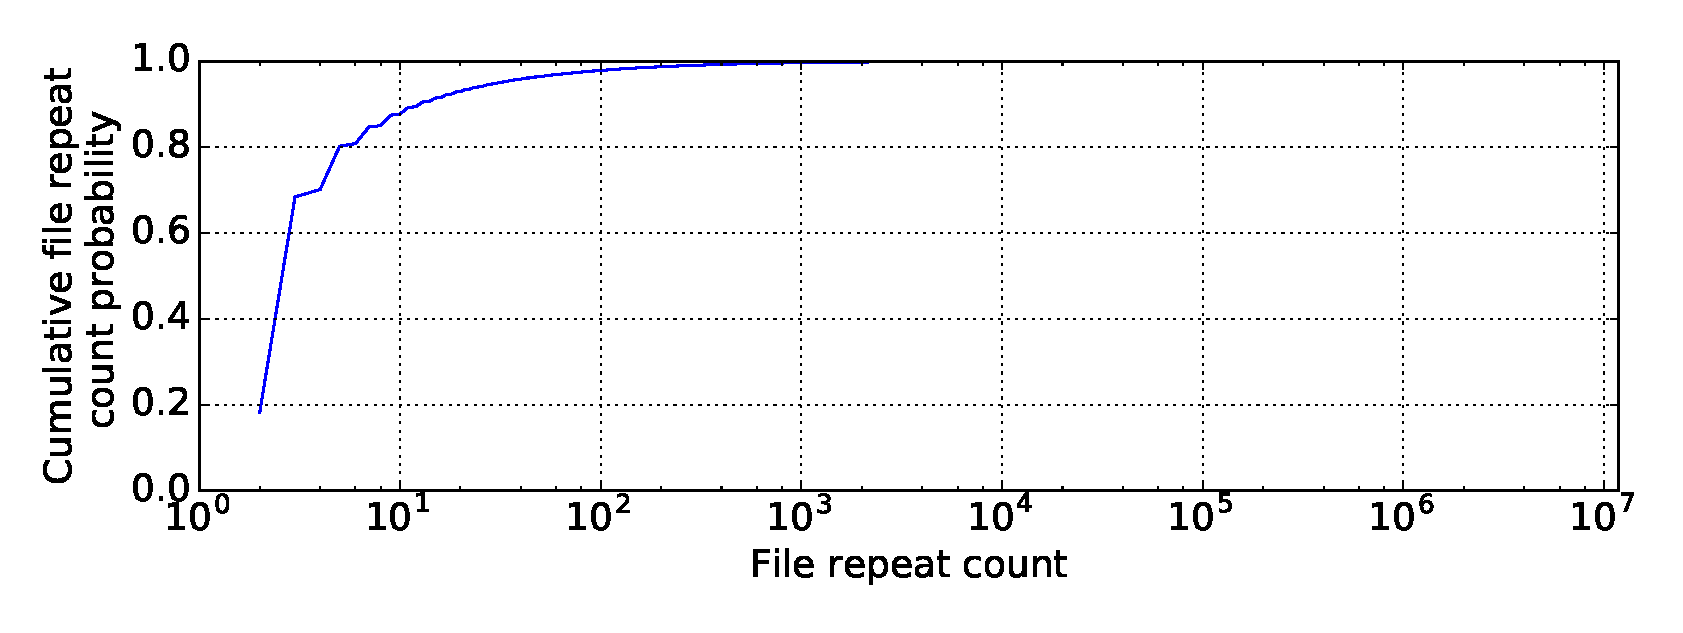
\includegraphics[width=0.5\textwidth]{graphs/File_repeat_count.eps}
	\caption{File repeat count distribution.
	}
	\label{fig:file-repeat-cnt}
\end{figure}

Figure~\ref{fig:file-repeat-cnt} shows the cumulative and probability distribution of file repeat count. 
Most files have a small repeat count. For instance, almost 90\% of files have equal or less than 10 copies. Around 50\% of files have 4 copies.
The file that has the maximum repeat count is empty file, which means that many users creates empty files and stored in their images.

Figure~\ref{fig:over-dup-overhead} shows the redundant file overhead of the uncompressed dataset in terms of file count and capacity. We see that only 0.58\% of files have a single copy while majority of the files have more than one copies. After file-level deduplication, the total number of duplicate files (i.e., repeat cnt. $>$ 1) decrease to 2.59\%. Consequently, only 3.17\% (23.92 TB) of files are unique files while 96.83\% of files (143.28 TB) are redundant copies, indicating that Docker Hub has severe redundancy problem. Table~\ref{tbl:overall-redundant_ratio} summaries the overall redundant file overhead in terms of file count and capacity.

Finding 1: Majority of files in registry are duplicates

\begin{figure}
	\centering
	\subfigure[Redundant file overhead in terms of file count]{\label{fig:over-dup-overhead-cnt}
		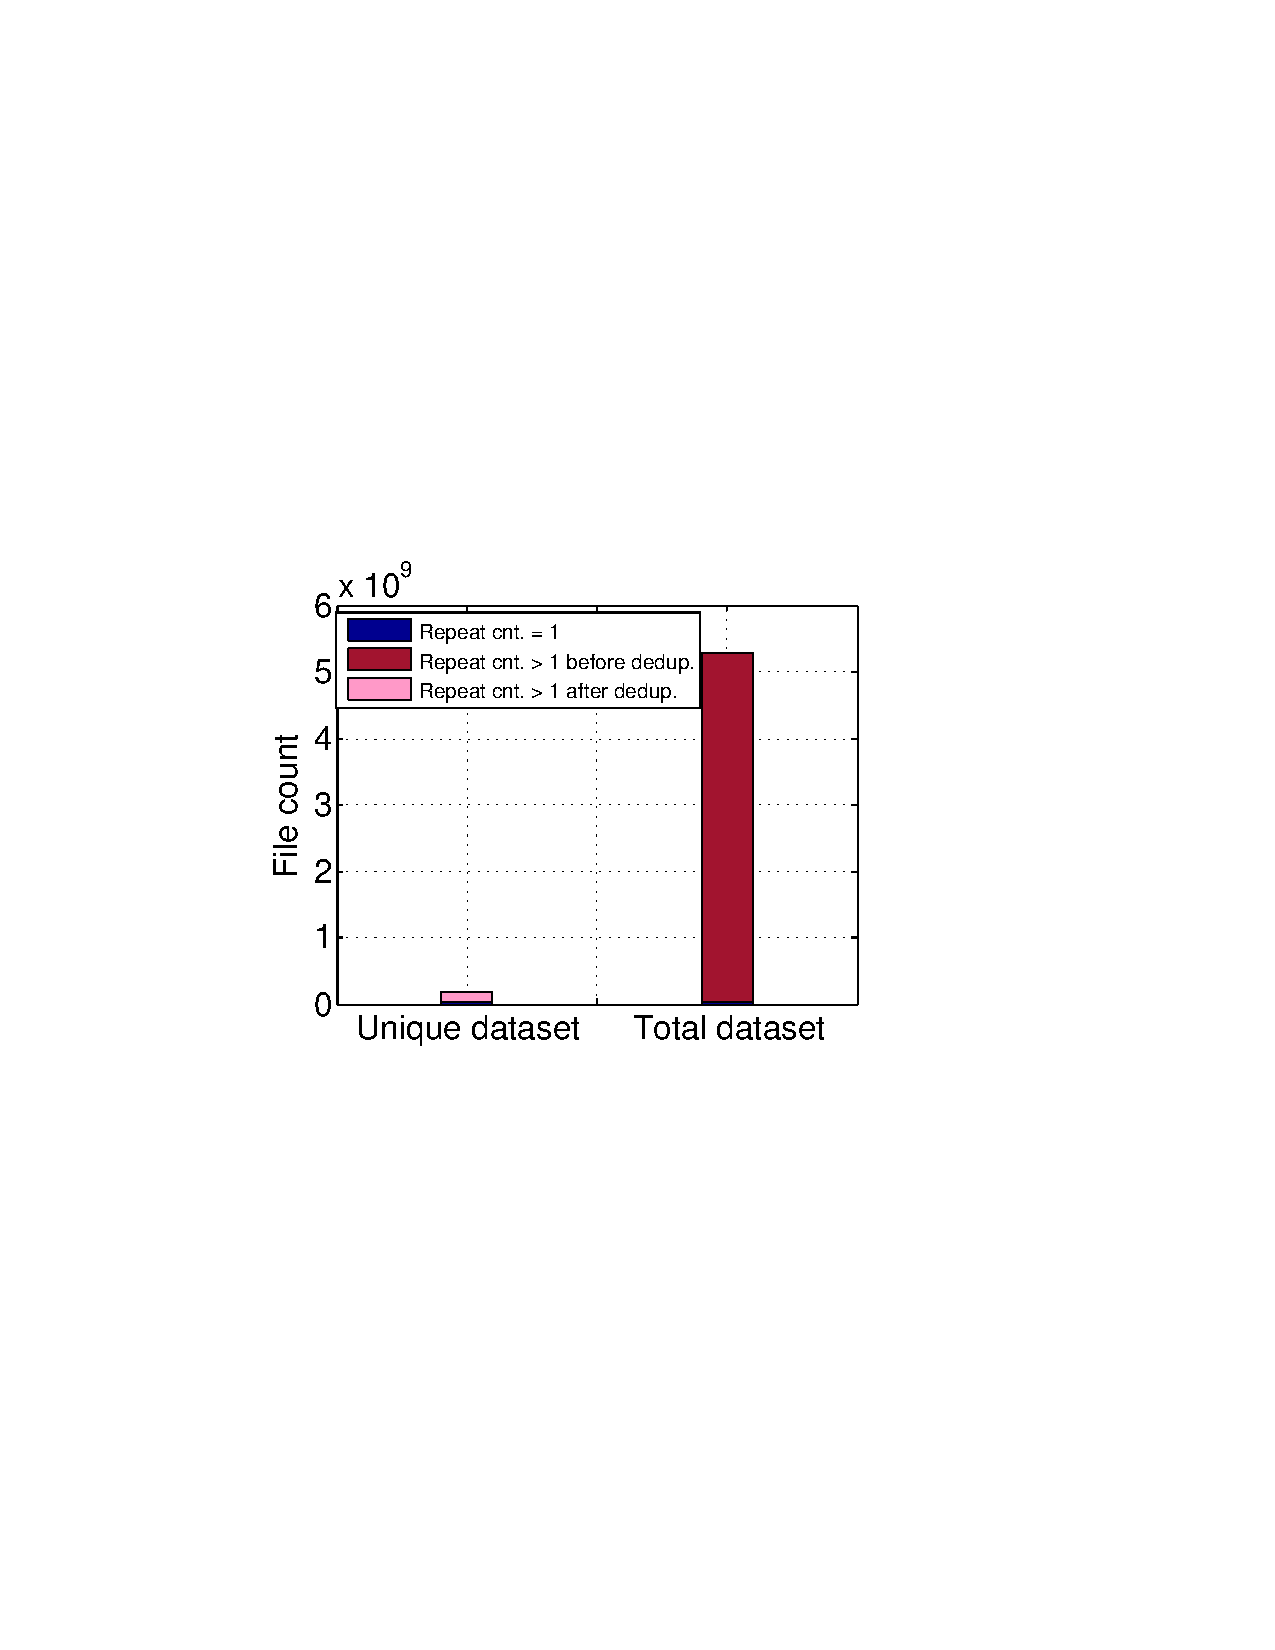
\includegraphics [width=0.21\textwidth]{graphs/dup-ratio-cnt.pdf}
	}
	\subfigure[Redundant file overhead in terms of capacity]{\label{fig:over-dup-overhead-cap}
		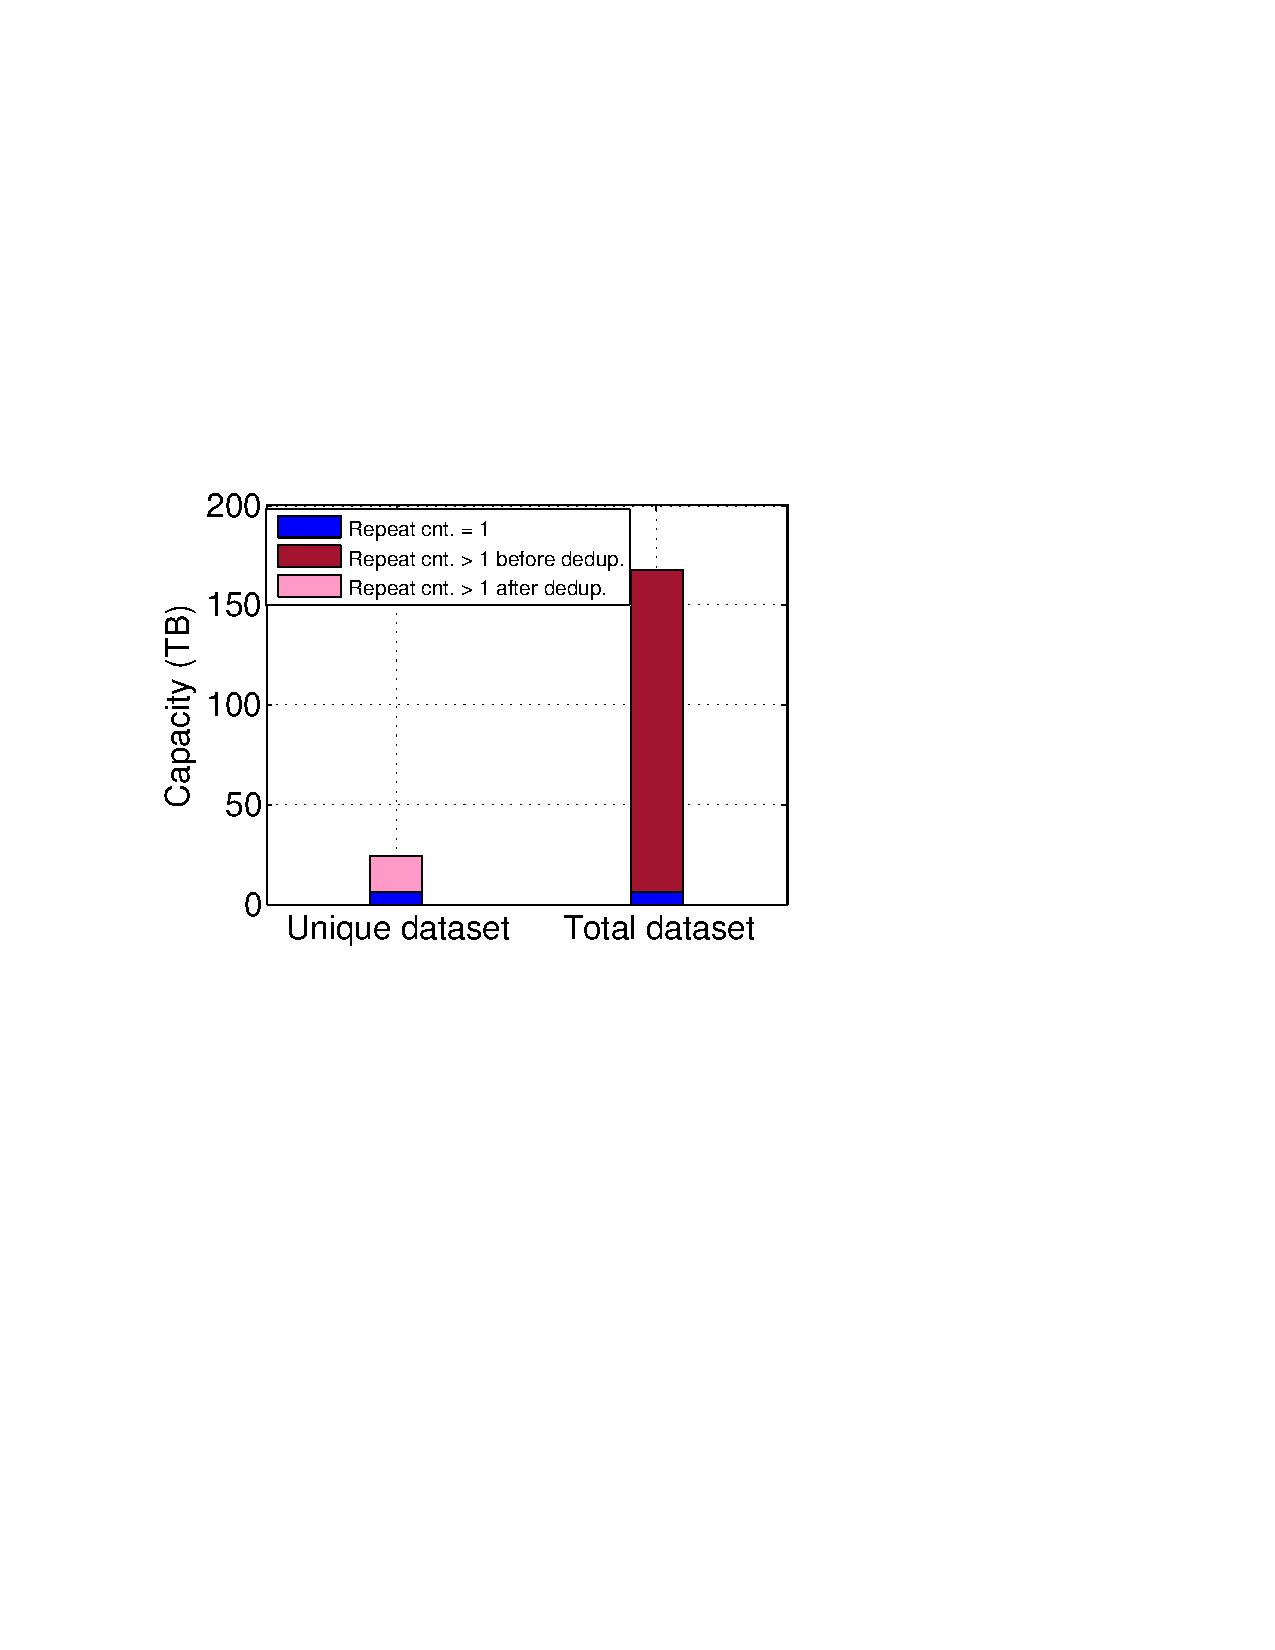
\includegraphics [width=0.225\textwidth]{graphs/dup-ratio-cap.pdf}
	}
	\caption{Redundant file overhead.}
	\label{fig:over-dup-overhead}
\end{figure}

\begin{table} 
	\centering 
	\scriptsize  
	%\begin{minipage}{.5\linewidth}
	\caption{Redundant ratio in terms of file count and capacity} \label{tbl:overall-redundant_ratio} 
	\begin{tabular}{|l|l|l|}%p{0.14\textwidth} 
		\hline  
		       & File count & Capacity \\
		\hline
		Repeat cnt = 1 & 0.58\% & 10.87\%\\
		\hline
		Repeat cnt $>$ 1 after dedup. & 2.59\% & 3.44\%\\
		\hline
		Repeat cnt $>$ 1 before dedup.  & 99.42\%  & 89.13\%\\
		\hline
		Unique dataset (Uncompressed) & 3.17\% (167,251,437)  &  14.31\% (23.92 TB) \\
		\hline 
		Total dataset (Uncompressed) & 5,278,465,130 & 167.20 TB \\
		\hline 	
		%\hline 
	\end{tabular} 
\end{table} 

%\subsection{Cross image sharing}

\paragraph{Cross image sharing}

Finding 2: There are a lot of duplicate files existing within individual layers and images while more duplicate files are stored across layers and images

We define two duplicate ratio for layers: intra-layer duplicate ratio and inter-layer duplicate ratio. Intra-layer duplicate ratio $r_{intra\_ldedup.}$ is calculated as:
$r_{intra\_ldedup.} = \frac{S_{un.\_l} - S_{un.\_ldedup.}}{S_{un.\_l}}$, where $S_{un.\_l}$ is the uncompressed layer size while $S_{un.\_ldedup.}$ is the uncompressed layer size after removing the intra-layer duplicate files. Inter-layer duplicate ratio $r_{inter\_ldedup.}$ is calculated as:
$r_{inter\_ldedup.} = \frac{S_{un.\_l} - S_{un.\_sldedup.}}{S_{un.\_l}}$, where $S_{un.\_l}$ is the uncompressed layer size while $S_{un.\_sldedup.}$ is the uncompressed layer size after removing the inter-layer duplicate files.

Figure~\ref{fig:layer-dedup-ratio} shows the intra/inter-layer duplicate ratio in terms of file count and capacity. As shown in Figure~\ref{fig:layer-dedup-cdf},
\nancomment{following description have problem.}
90\% of layers contains less than 53\% of intra-layer redundant files while 90\% of layers contains bigger than 97.6\% of inter-layer redundant files, indicating that majority of files are replicated across different layers and plenty of redundant files are replicated within each layer.
Figure~\ref{fig:layer-dedup_hist} shows that 1.1 M of layers contains 45\% of the intra-layer duplicate files. We manually inspect few of these layers and found xxxx.
While 1.5 M of layers contains 95\% of the inter-layer duplicate files. We also manually inspect few of these layers that found xxx.

As shown in Figure~\ref{fig:layer-dedup-ratio}, the differences between  duplicate ratio in terms of file count and  duplicate ratio in terms of capacity are very small, meaning that there is no huge difference among the sizes of duplicate files.

Similar to images, we also calculated the intra-image duplicate ratio and inter-image duplicate ratio. Figure~\ref{fig:image-dedup-ratio} shows the intra/inter-image duplicate ratio in terms of file count and capacity. 
90\% of images contains less than 54.4\% of intra-image redundant files while 90\% of images contains bigger than 99.4\% of inter-image redundant files, indicating that majority of files are replicated across different images and plenty of redundant files are replicated within each image.
Figure~\ref{fig:layer-dedup_hist} shows that 0.2 M of images contains 0.45 of the intra-image duplicate files. We manually inspect few of these images and found xxxx.
While 0.3 M of images contains 95\% of the inter-image duplicate files. We also manually inspect few of these layers that found xxx.

Interestingly, we fond that considerable duplicate files are stored across the layers referred by the same images.

\nancomment{inspecting the layers and images with 0.45 dup ratio}
\nancomment{get the dup ratio for layers that are referred by same images, if have time}

%\begin{eqnarray}
%$r_{inter\_dedup.} = \frac{S_{uncompress.} - S_{shares}}{S_{uncompress.}}$
%\end{eqnarray}

%\paragraph{Intra-layer redundant ratio} Intra-layer redundant ratio is shown in .
\begin{figure}
	\centering
	\subfigure[CDF of intra/inter-layer redundant ratio in terms of file count(denoted as *-cnt.)/capacity(denoted as *-cap.)]{\label{fig:layer-dedup-cdf}
		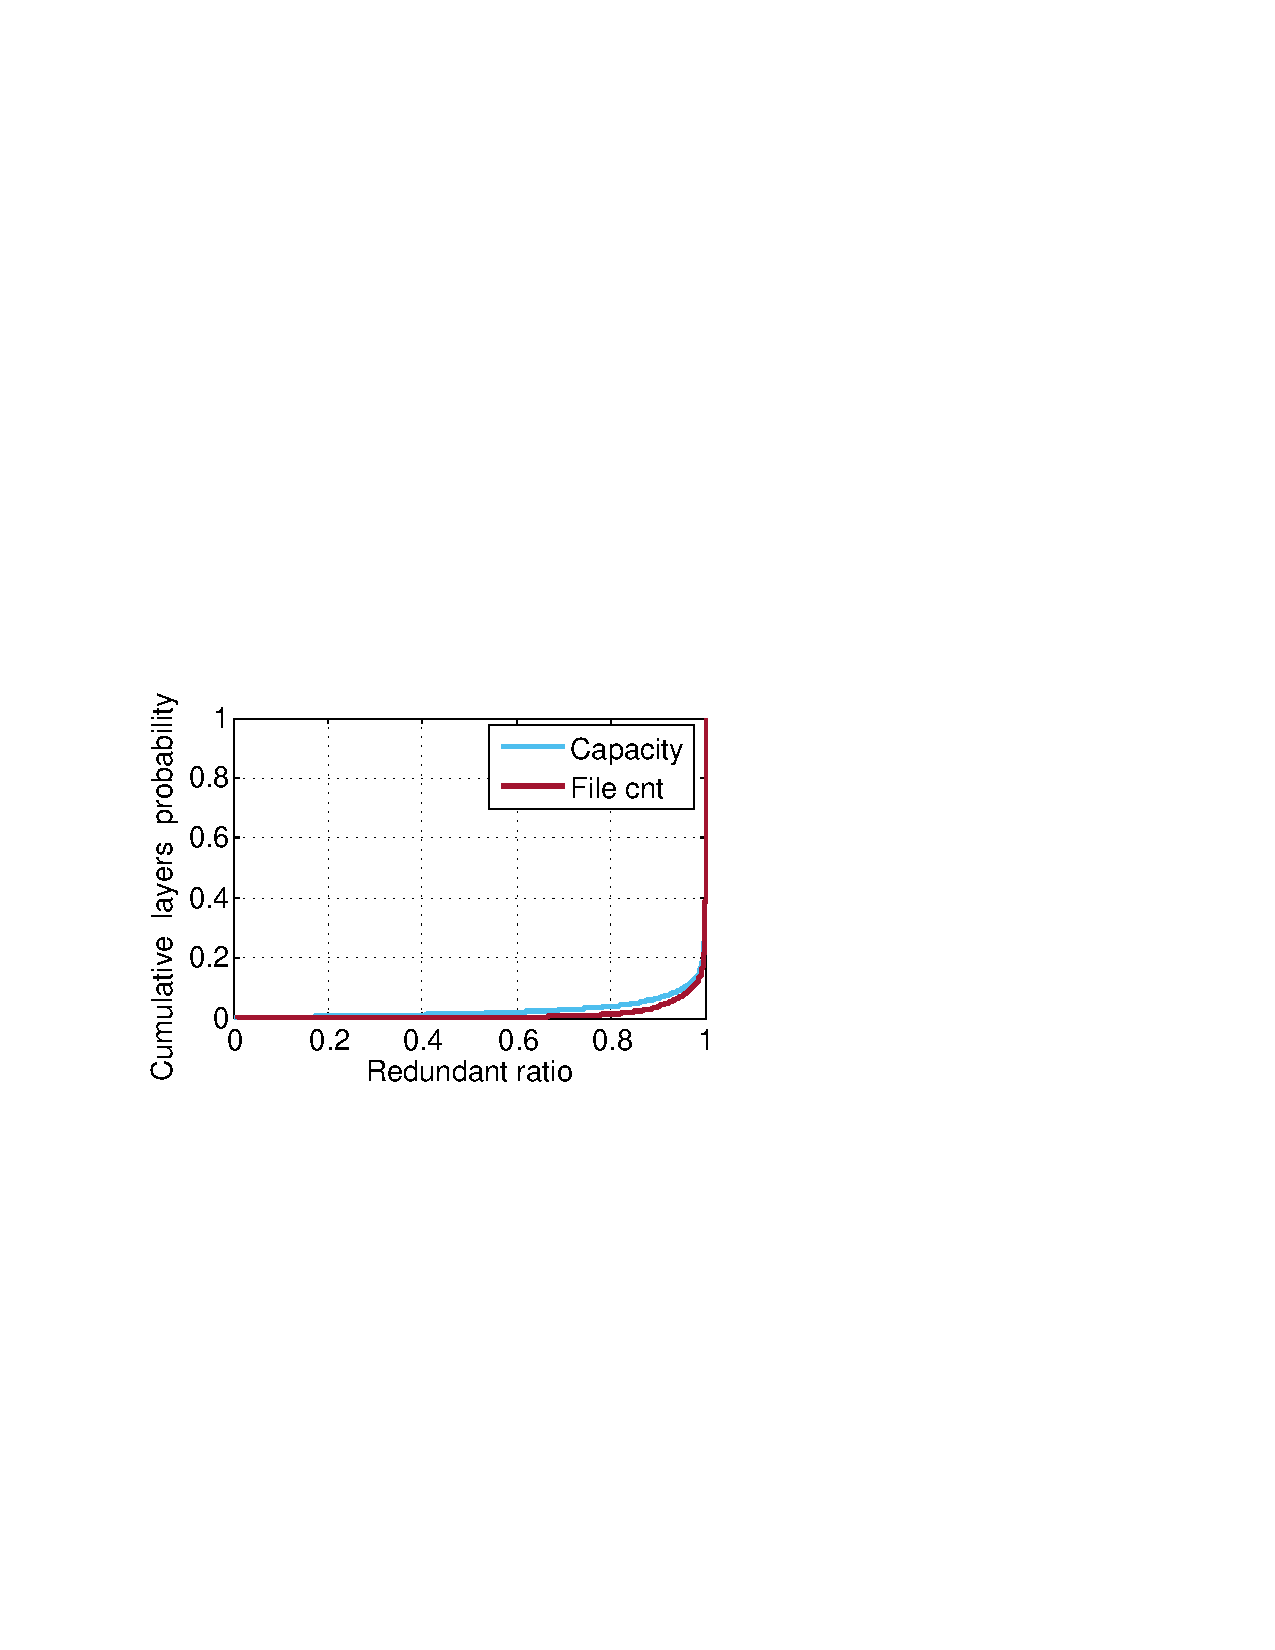
\includegraphics [width=0.4\textwidth]{graphs/layer-dup-ratio-cdf}
	}
	\subfigure[Histogram of intra/inter-layer redundant ratio in terms of file count(denoted as *-cnt.)/capacity(denoted as *-cap.)]{\label{fig:layer-dedup_hist}
		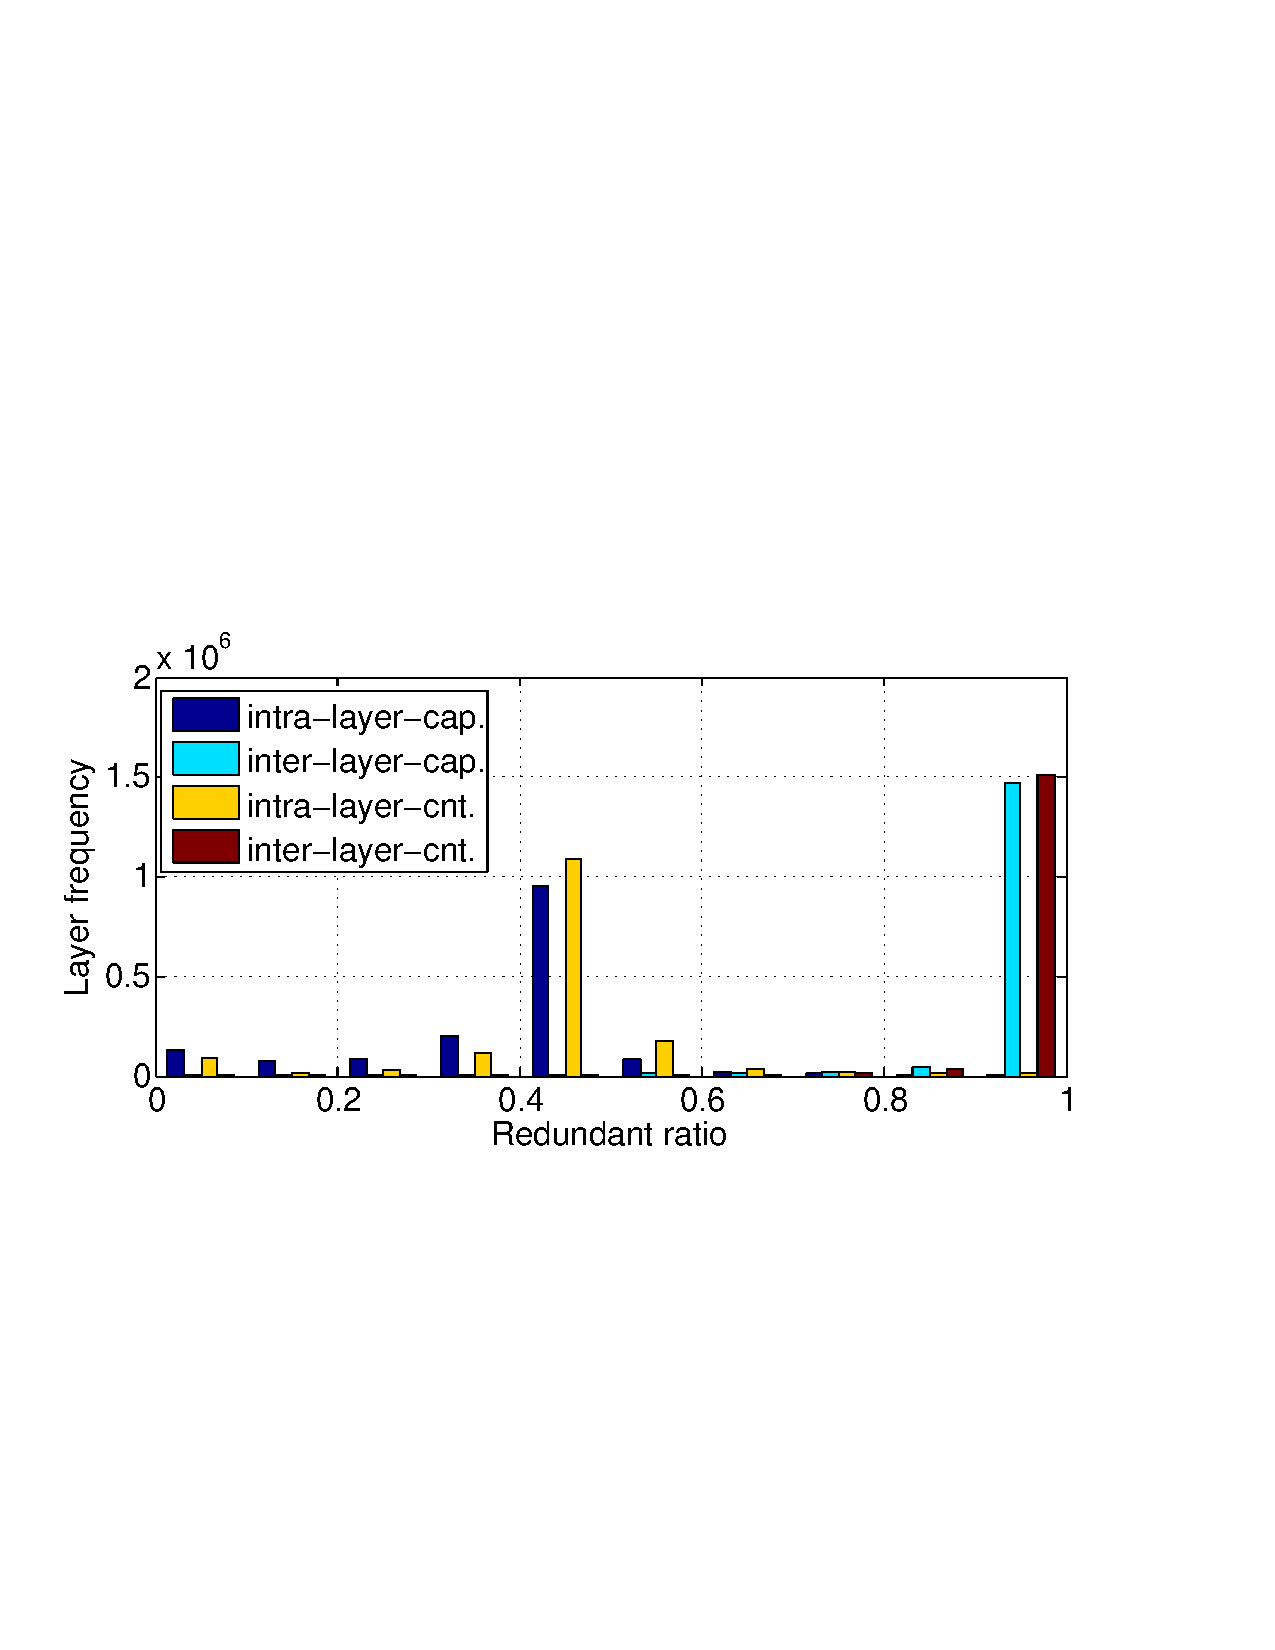
\includegraphics [width=0.4\textwidth]{graphs/layer-dup-ratio-pdf}
	}
	\caption{Layer redundant ratio}
	\label{fig:layer-dedup-ratio}
\end{figure}

%\paragraph{Inter-layer redundant ratio} Inter-layer redundant ratio is shown in Figure~\ref{fig:layer-dedup-ratio}

%\subsection{Redundant ratio for images}
%\paragraph{Finding 3: Similar to layer, \% of images contains \% of inter-image redundant files and \% of image contains \% of intra-image redundant files, indicating that large amount of files are replicated across different images and plenty of redundant files are replicated within each image}

\begin{figure}
	\centering
	\subfigure[CDF of intra/inter-image redundant ratio in terms of file count(denoted as *-cnt.)/capacity(denoted as *-cap.)]{\label{fig:image-dedup_cdf}
		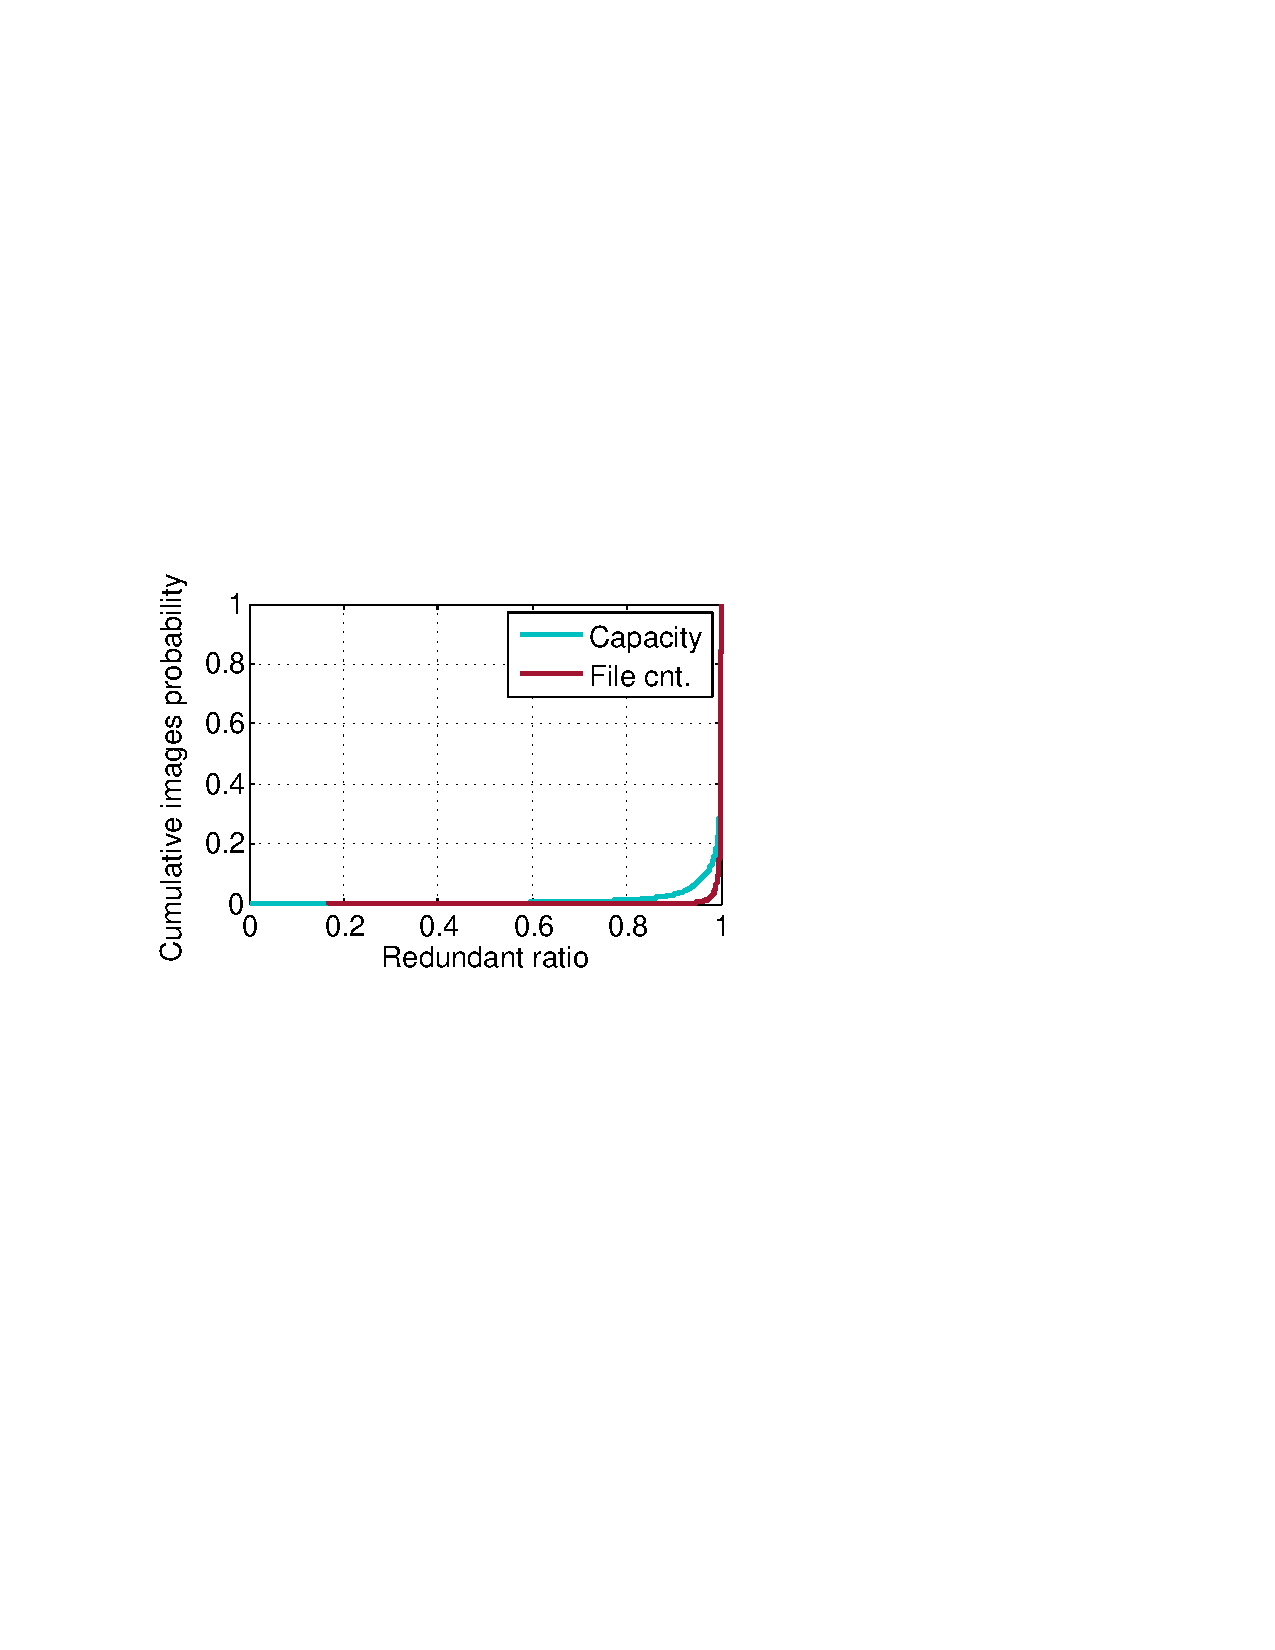
\includegraphics [width=0.4\textwidth]{graphs/image-dup-ratio-pdf}
	}
	\subfigure[Histogram of intra/inter-image redundant ratio in terms of file count(denoted as *-cnt.)/capacity(denoted as *-cap.)]{\label{fig:image-dedup_hist}
		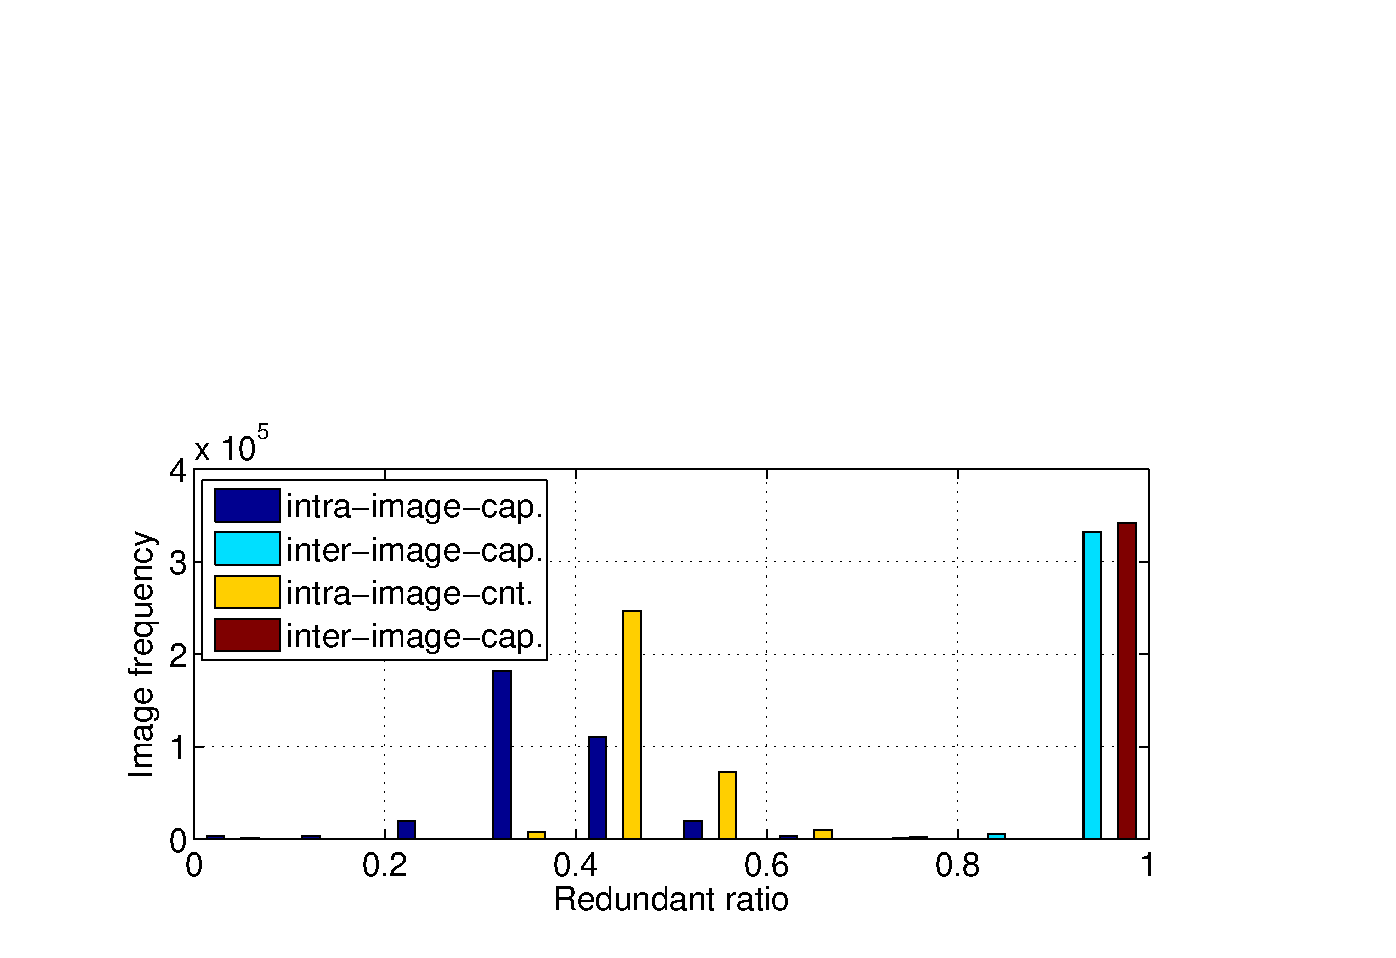
\includegraphics [width=0.4\textwidth]{graphs/image-dup-ratio-cdf}
	}
	\caption{Image redundant ratio}
	\label{fig:image-dedup-ratio}
\end{figure}


%\paragraph{Intra-image redundant ratio} Intra-image redundant ratio is shown in Figure~\ref{fig:image-dedup-ratio}

%\paragraph{Inter-image redundant ratio} Inter-image redundant ratio is shown in Figure~\ref{fig:image-dedup-ratio}


%=======================================
%|             OLD VERSION              |
%=======================================
%\subsubsection{Overview of redundant ratio for layers}
%\begin{table} 
%	\centering 
%	\scriptsize  
%	%\begin{minipage}{.5\linewidth}
%	\caption{Intra-layer redundant ratio for layers in terms of file count and capacity} \label{tbl:intra_dup_ratio_layers} 
%	\begin{tabular}{|l|l|l|}%p{0.14\textwidth} 
%		\hline 
%		% after \\: \hline or \cline{col1-col2} \cline{col3-col4} ... 
%		% after \\: \hline or \cline{col1-col2} \cline{col3-col4} ... 
%		& File count & Capacity \\
%		\hline
%		Avg. & 49.78\% & 40.09\%\\
%		\hline
%		Median & - & - \\
%		\hline
%		Max. & 99.99\% & 99.99\%\\
%		\hline
%		Min.  & 0.00\%  & 0.00\%\\
%		\hline
%		Stdev.  &  2.14\% & 17.18\%\\
%		\hline
%		Layer dataset after intra.-dedup (Uncompressed) & -  & -\\
%		\hline 
%		Total layer dataset (Uncompressed) &  -	& -\\
%		\hline 
%		%\hline 
%	\end{tabular} 
%\end{table}

%\begin{table} 
%	\centering 
%	\scriptsize  
%	%\begin{minipage}{.5\linewidth}
%	\caption{Inter-layer redundant ratio for layers in terms of file count and capacity} \label{tbl:inter_dup_ratio_layers} 
%	\begin{tabular}{|l|l|l|}%p{0.14\textwidth} 
%		\hline 
%		% after \\: \hline or \cline{col1-col2} \cline{col3-col4} ... 
%		% after \\: \hline or \cline{col1-col2} \cline{col3-col4} ... 
%		& File count & Capacity \\
%		\hline
%		Avg. & 98.75\% & 97.33\%\\
%		\hline
%		Median & - & - \\
%		\hline
%		Max. & 1 & 1\\
%		\hline
%		Min.  & 0.87\%  & $<$ 0.00\%\\
%		\hline
%		Stdev.  &  4.70\% & 10.49\\
%		\hline
%		Layer dataset after inter.-dedup (Uncompressed) & -  & -\\
%		\hline 
%		Total layer dataset (Uncompressed) &  -	& -\\
%		\hline
%	\end{tabular} 
%\end{table}

%\subsubsection{Redundant ratio distribution}

%\paragraph{Cumulative distribution for intra-layer redundant ratio and inter-layer redundant ratio in terms of file count and storage capacity}



%\paragraph{Intra-layer redundant ratio by layer size in terms of file count and storage capacity}

%\begin{figure}
%	\centering
%	\includegraphics[width=0.5\textwidth]{graphs/inter-dedup-by-size.eps}
%	\caption{Intra-layer redundant ratio by layer size.
%	}
%	\label{fig_redundant_overhead}
%\end{figure}

%\subsubsection{Inter-layer redundant overhead}

%\paragraph{Histogram of intra-layer redundant ratio and inter-layer redundant ratio in terms of file count and storage capacity}

%\paragraph{Inter-layer redundant ratio by layer size in terms of file count and storage capacity}

%\subsubsection{Overview of redundant ratio for images}

%\begin{table} 
%	\centering 
%	\scriptsize  
%	%\begin{minipage}{.5\linewidth}
%	\caption{Inter-layer redundant ratio for images in terms of file count and capacity} \label{tbl:intra_dup_ratio_images} 
%	\begin{tabular}{|l|l|l|}%p{0.14\textwidth} 
%		\hline 
%		% after \\: \hline or \cline{col1-col2} \cline{col3-col4} ... 
%		% after \\: \hline or \cline{col1-col2} \cline{col3-col4} ... 
%		& File count & Capacity \\
%		\hline
%		Avg. & 98.75\% & 97.33\%\\
%		\hline
%		Median & - & - \\
%		\hline
%		Max. & 1 & 1\\
%		\hline
%		Min.  & 0.87\%  & $<$ 0.00\%\\
%		\hline
%		Stdev.  &  4.70\% & 10.49\\
%		\hline
%		Layer dataset after share.-dedup (Uncompressed) & -  & -\\
%		\hline 
%		Total layer dataset (Uncompressed) &  -	& -\\
%		\hline
%	\end{tabular} 
%\end{table}
%
%\begin{table} 
%	\centering 
%	\scriptsize  
%	%\begin{minipage}{.5\linewidth}
%	\caption{Intra-layer redundant ratio for images in terms of file count and capacity} \label{tbl:inter_dup_ratio_images} 
%	\begin{tabular}{|l|l|l|}%p{0.14\textwidth} 
%		\hline 
%		% after \\: \hline or \cline{col1-col2} \cline{col3-col4} ... 
%		% after \\: \hline or \cline{col1-col2} \cline{col3-col4} ... 
%		& File count & Capacity \\
%		\hline
%		Avg. & 98.75\% & 97.33\%\\
%		\hline
%		Median & - & - \\
%		\hline
%		Max. & 1 & 1\\
%		\hline
%		Min.  & 0.87\%  & $<$ 0.00\%\\
%		\hline
%		Stdev.  &  4.70\% & 10.49\\
%		\hline
%		Layer dataset after share.-dedup (Uncompressed) & -  & -\\
%		\hline 
%		Total layer dataset (Uncompressed) &  -	& -\\
%		\hline
%	\end{tabular} 
%\end{table}

%\subsubsection{Redundant ratio distribution}
%\paragraph{Cumulative distribution for intra-image redundant ratio and inter-image redundant ratio in terms of file count and storage capacity}
%\paragraph{Histogram of intra-image redundant ratio and inter-image redundant ratio in terms of file count and storage capacity}

